% !TEX root = ../main.tex
\chapter{Triển khai hệ thống}

\section{Tổ chức mã nguồn và phạm vi triển khai}

RabbitCV được triển khai theo kiến trúc web client--server. Mã nguồn được tổ chức thành các phần chính sau:

\begin{itemize}
    \item \textbf{Frontend:} nằm trong thư mục \texttt{src}, bao gồm page, component, context, hook và utility.
    \item \textbf{Backend:} nằm trong thư mục \texttt{server}, bao gồm Express entry point, model Mongoose, route AI, service AI, utility kiểm tra dữ liệu và tác vụ định kỳ.
    \item \textbf{Giao tiếp giữa hai phần:} chủ yếu sử dụng REST API; riêng thông điệp chat được phát thêm qua Socket.IO sau khi server lưu dữ liệu thành công.
\end{itemize}

\begin{table}[H]
    \centering
    \small
    \begin{tabularx}{\textwidth}{|p{0.18\textwidth}|p{0.31\textwidth}|Y|} \hline
        \textbf{Lớp} & \textbf{Thành phần tiêu biểu} & \textbf{Trách nhiệm đã triển khai} \\ \hline
        Giao diện & Page, component, React Router & Điều hướng, nhập liệu, preview CV, hiển thị Job, hồ sơ, chat và kết quả AI. \\ \hline
        Trạng thái dùng chung & AuthContext, SavedJobsContext, SocketContext, QueryClient & Phiên đăng nhập, cache việc đã lưu/thông báo, cập nhật lạc quan và kết nối sự kiện chat. \\ \hline
        Nền tảng giao diện & Form schema, Radix UI, Sonner, Error Boundary & Kiểm tra biểu mẫu, hộp thoại/menu có portal, phản hồi thao tác và phục hồi lỗi kết xuất. \\ \hline
        API nghiệp vụ & Express routes trong \texttt{server.js} & Xác thực, Resume, Job, Application, Message, Notification, saved jobs và admin. \\ \hline
        API AI & \texttt{aiRoutes.js}, \texttt{aiService.js} & Năm workflow AI, quota, rate limit, timeout, structured output và ghi nhận usage. \\ \hline
        Dữ liệu & Chín model Mongoose & User, Resume, Job, Application, Message, Notification, HiddenChat, ChatReadState và AiUsage. \\ \hline
        Kiểm tra biên & Utility sanitizer/validator & Kiểm tra PDF, rich text CV, ngày, khả dụng của Job và dữ liệu gửi/nhận từ AI. \\ \hline
    \end{tabularx}
    \caption{Ánh xạ các lớp triển khai của RabbitCV}
    \label{tab:implementation-layers}
\end{table}

Frontend nạp lười nhiều trang để giảm lượng mã ban đầu và Vite chia các thư viện lớn thành nhóm riêng. Backend hiện vẫn tập trung phần lớn route nghiệp vụ trong \texttt{server.js}; cách tổ chức này phù hợp bản đồ án nhưng là một giới hạn bảo trì được thảo luận ở Chương 7 và Chương 8.

\section{Xác thực và phân quyền}

Route đăng ký kiểm tra username, email, mật khẩu và vai trò trước khi tạo User; mật khẩu được băm bằng bcryptjs. Route đăng nhập tạo JWT có thời hạn một ngày hoặc 30 ngày theo lựa chọn ghi nhớ và gửi token qua cookie HTTP-only. Khi ứng dụng khởi động hoặc tải lại, \texttt{AuthContext} dùng bản sao trong \texttt{sessionStorage} cho phản hồi ban đầu, đồng thời gọi \texttt{/api/me} để xác nhận phiên và cung cấp \texttt{currentUser} cho cây component.

Biểu mẫu đăng nhập và đăng ký sử dụng React Hook Form cùng Zod để kiểm tra trường bắt buộc, email, xác nhận mật khẩu, vai trò và điều khoản. Ở frontend, \texttt{RoleAccessGuard} điều hướng doanh nghiệp và quản trị viên về cổng tương ứng; Error Boundary ở gốc cho phép tải lại khi lỗi React không được xử lý. Ở backend, middleware xác thực đọc token và các route đặc quyền kiểm tra vai trò hoặc quan hệ sở hữu. Frontend guard chỉ cải thiện trải nghiệm; quyết định cho phép đọc hoặc thay đổi dữ liệu luôn phải được thực hiện ở server.

\begin{figure}[H]
    \centering
    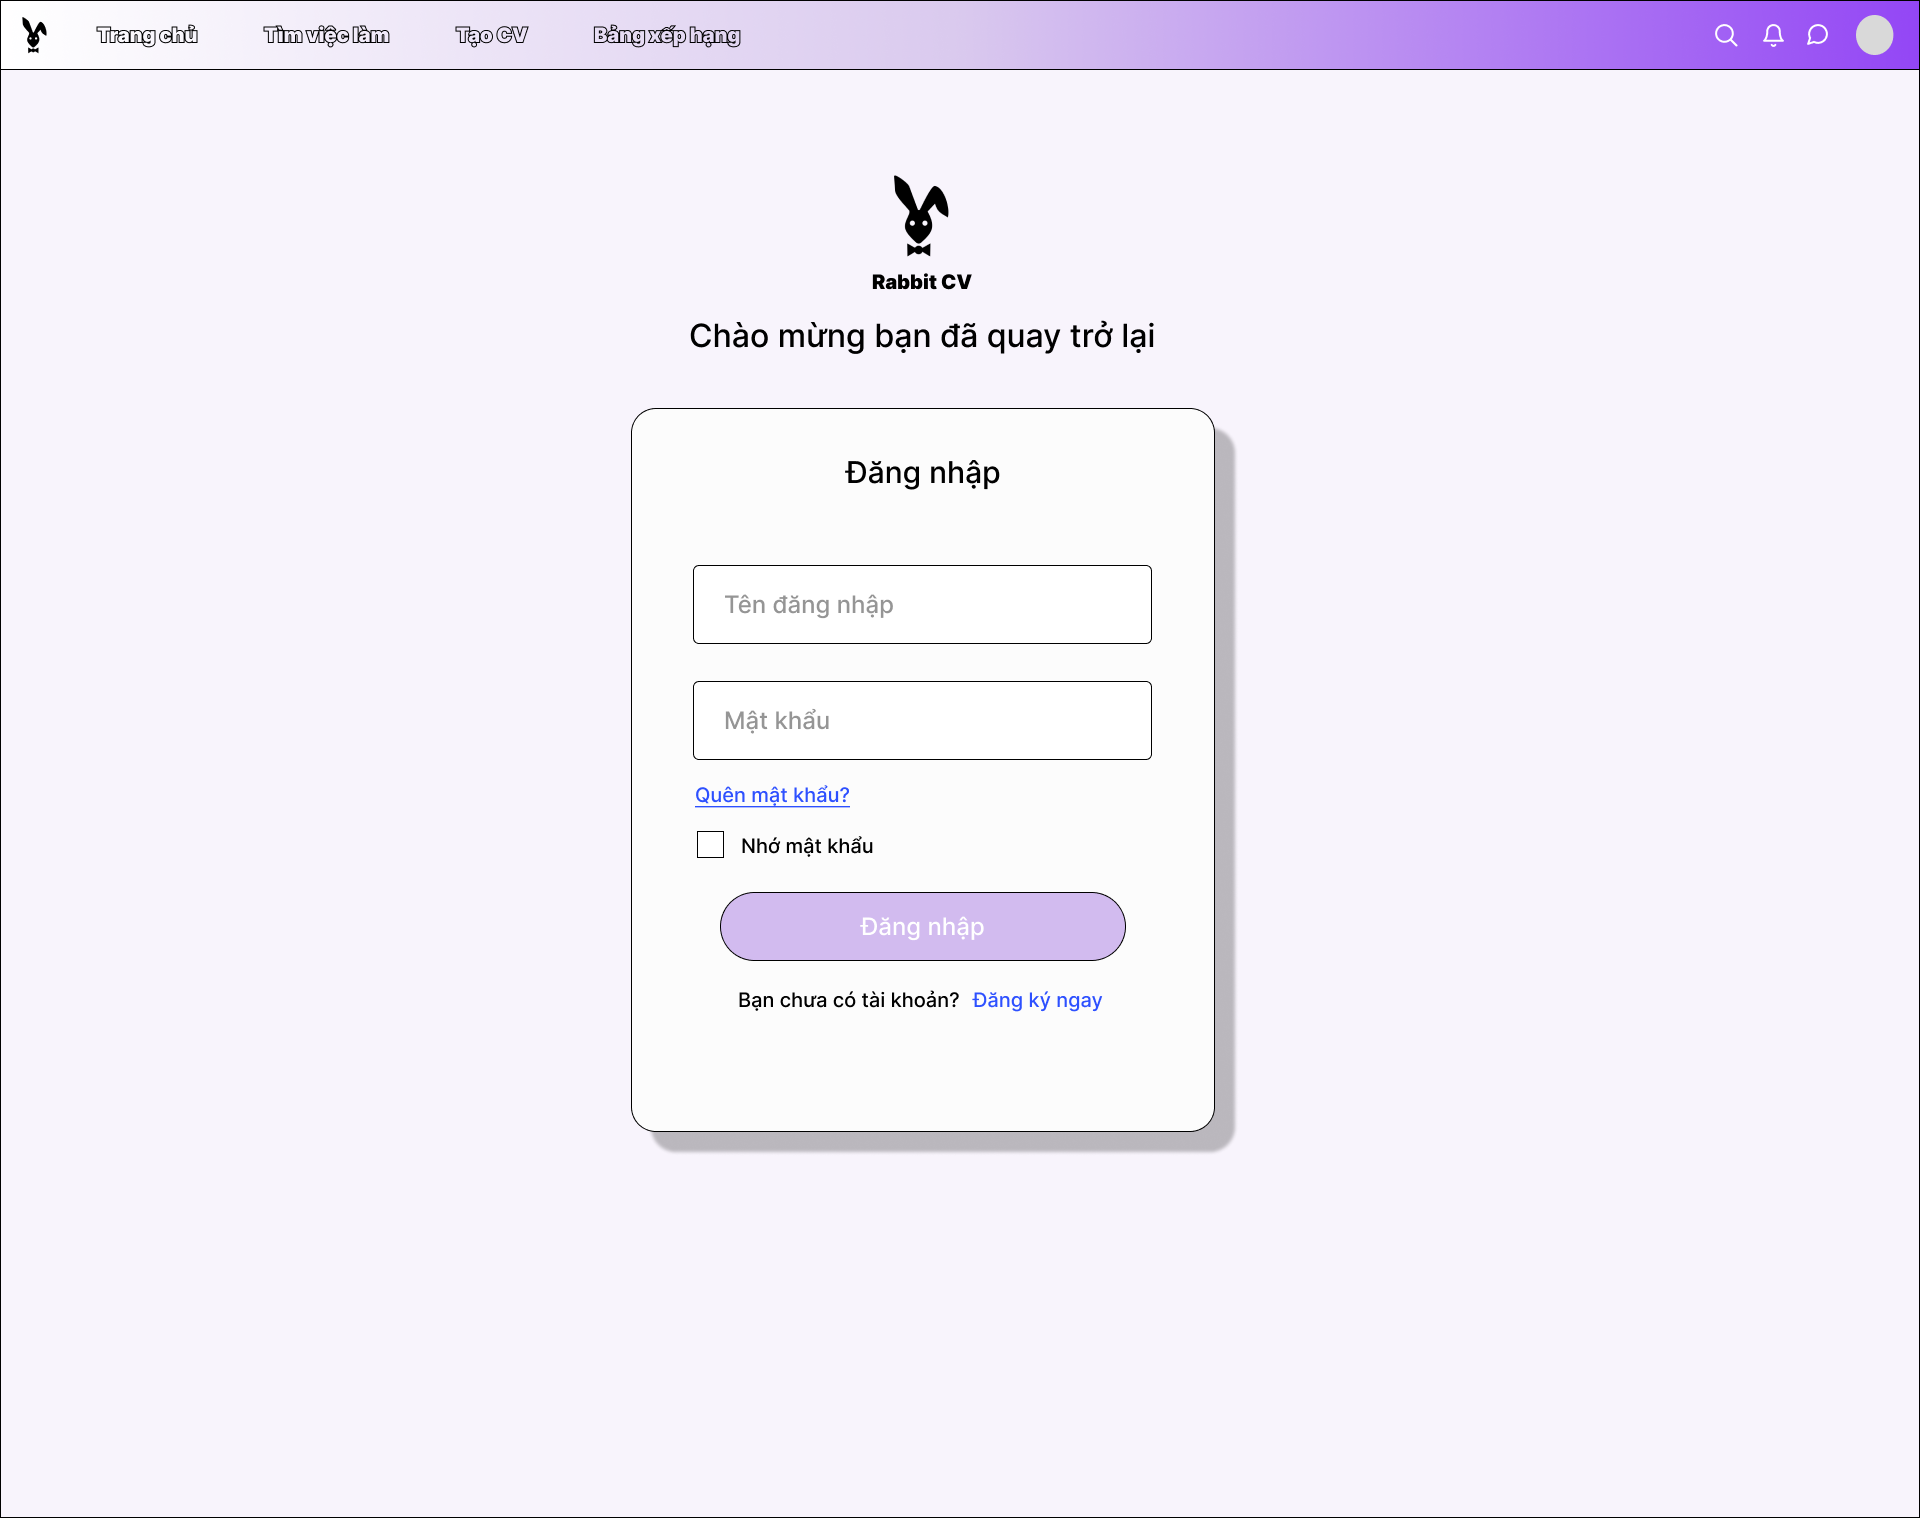
\includegraphics[width=0.83\textwidth]{img/Login.png}
    \caption{Giao diện đăng nhập của RabbitCV}
    \label{fig:login}
\end{figure}

\section{Tạo, quản lý và xuất CV}

Resume lưu dữ liệu có cấu trúc theo các nhóm thông tin cá nhân, tiểu sử, kinh nghiệm, học vấn, kỹ năng, dự án, chứng chỉ, ngôn ngữ, giải thưởng và sở thích. Cách lưu này cho phép người dùng đổi template, tiếp tục chỉnh sửa và tái tạo bản trình bày mà không phải phân tích ngược một file PDF.

\begin{figure}[H]
    \centering
    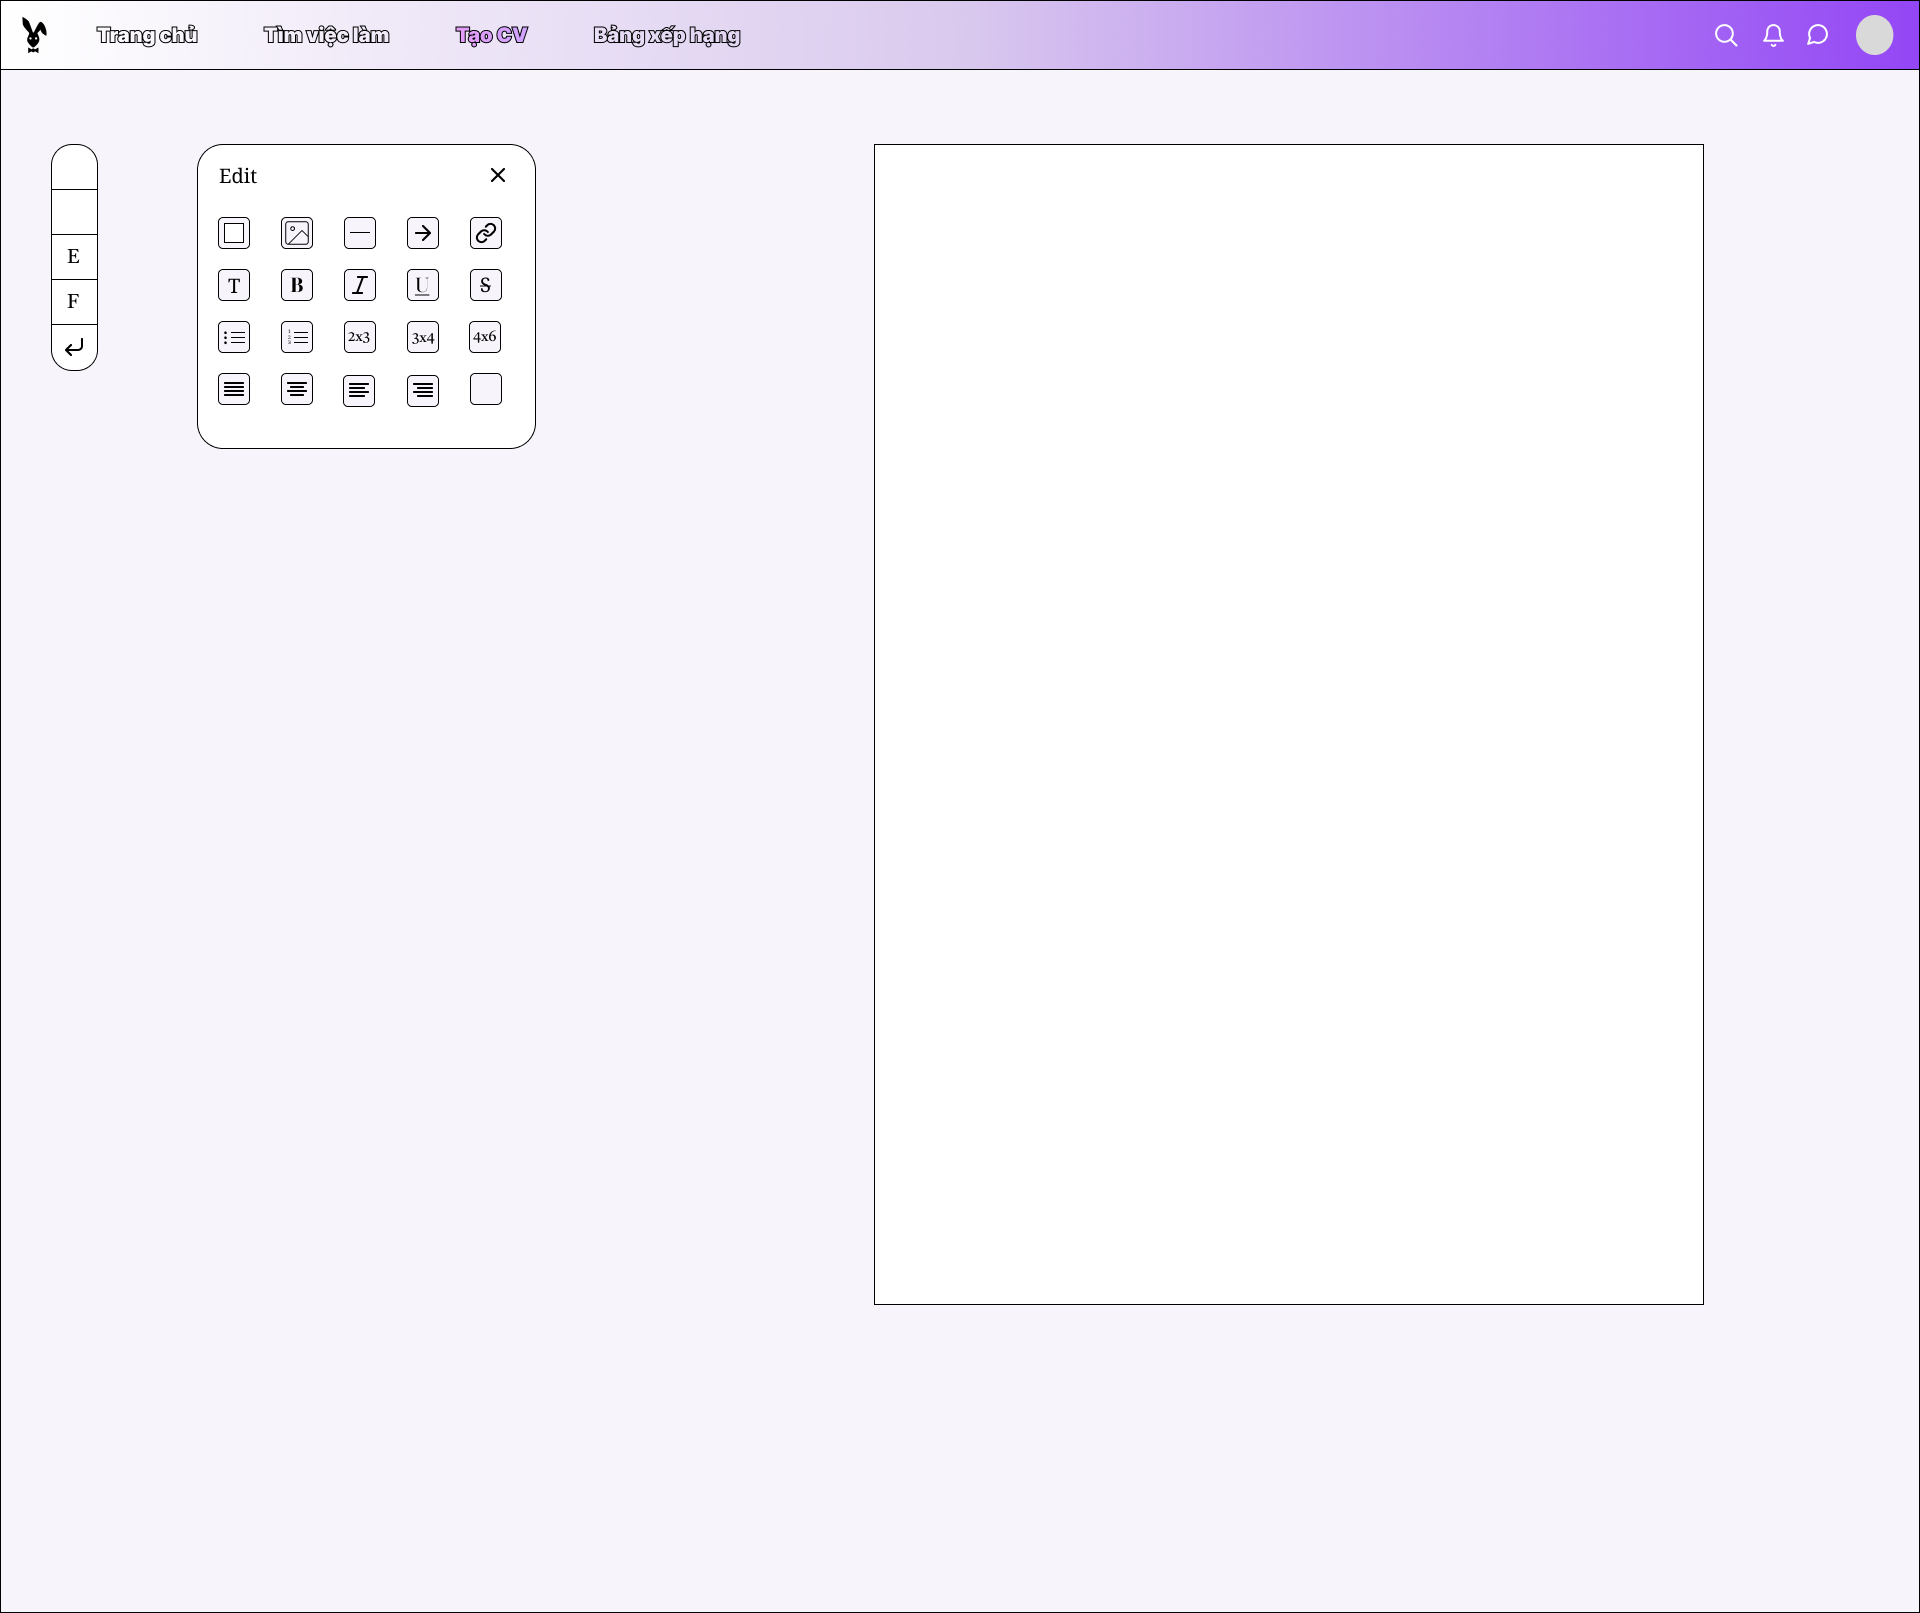
\includegraphics[width=0.92\textwidth]{img/CV_Management.png}
    \caption{Khung chỉnh sửa và vùng preview CV}
    \label{fig:cv-management}
\end{figure}

Các vùng mô tả dùng Tiptap. Khi lưu, backend làm sạch HTML theo danh sách thẻ cho phép; khi hiển thị, static renderer chuyển nội dung thành phần tử React thay vì chèn chuỗi HTML trực tiếp. Preview CV dùng khung có kích thước vật lý A4 và quy tắc CSS dành cho in. Hook \texttt{useResumePrint} dựa trên \texttt{react-to-print} được dùng chung ở trình biên tập và thư viện CV, đặt tiêu đề tệp, CSS trang in và xử lý lỗi. Với CV tải lên trong luồng ứng tuyển, backend kiểm tra data URL, MIME, phần mở rộng, header PDF và dung lượng giải mã tối đa 5~MB. PDF được hiển thị theo từng trang bằng PDF.js thay vì dùng iframe của trình duyệt.

Hai quyết định dữ liệu giúp luồng CV ổn định hơn. Thứ nhất, \texttt{isVirtual} phân biệt Resume dùng tạm trong một Application với CV do người dùng quản lý. Thứ hai, endpoint danh sách loại \texttt{pdfData} khỏi kết quả để tránh tải toàn bộ file base64 khi chỉ cần metadata. Endpoint xem CV kiểm tra quyền sở hữu hoặc quan hệ tuyển dụng trước khi trả nội dung.

\section{Tích hợp AI có kiểm soát}

Nhóm route \texttt{/api/ai} cung cấp năm chức năng:

\begin{itemize}
    \item viết hoặc cải thiện phần giới thiệu;
    \item rà soát CV;
    \item gợi ý điền các mục còn thiếu;
    \item so khớp CV với công việc;
    \item luyện tập phỏng vấn.
\end{itemize}

Tất cả yêu cầu đều đi qua backend nên khóa truy cập nhà cung cấp không xuất hiện trong frontend. Kết quả được hiển thị dưới dạng gợi ý và chỉ làm thay đổi CV khi người dùng chủ động áp dụng.

Kiến trúc, hợp đồng API, quy trình làm sạch dữ liệu, đầu ra có cấu trúc, hạn mức và thống kê sử dụng được trình bày riêng tại Chương~\ref{chap:ai-module}.

\section{Tìm việc và ứng tuyển}

Endpoint danh sách Job là tài nguyên công khai; giao diện hỗ trợ tìm từ khóa, công ty, địa điểm và thẻ, đồng thời phân biệt trạng thái tin. Với người dùng đã đăng nhập, SavedJobsContext giữ giao diện dùng chung nhưng dữ liệu được quản lý bằng TanStack Query. Thao tác lưu/bỏ lưu cập nhật cache lạc quan, khôi phục trạng thái cũ khi API thất bại và làm mới lại sau khi hoàn tất.

\begin{figure}[H]
    \centering
    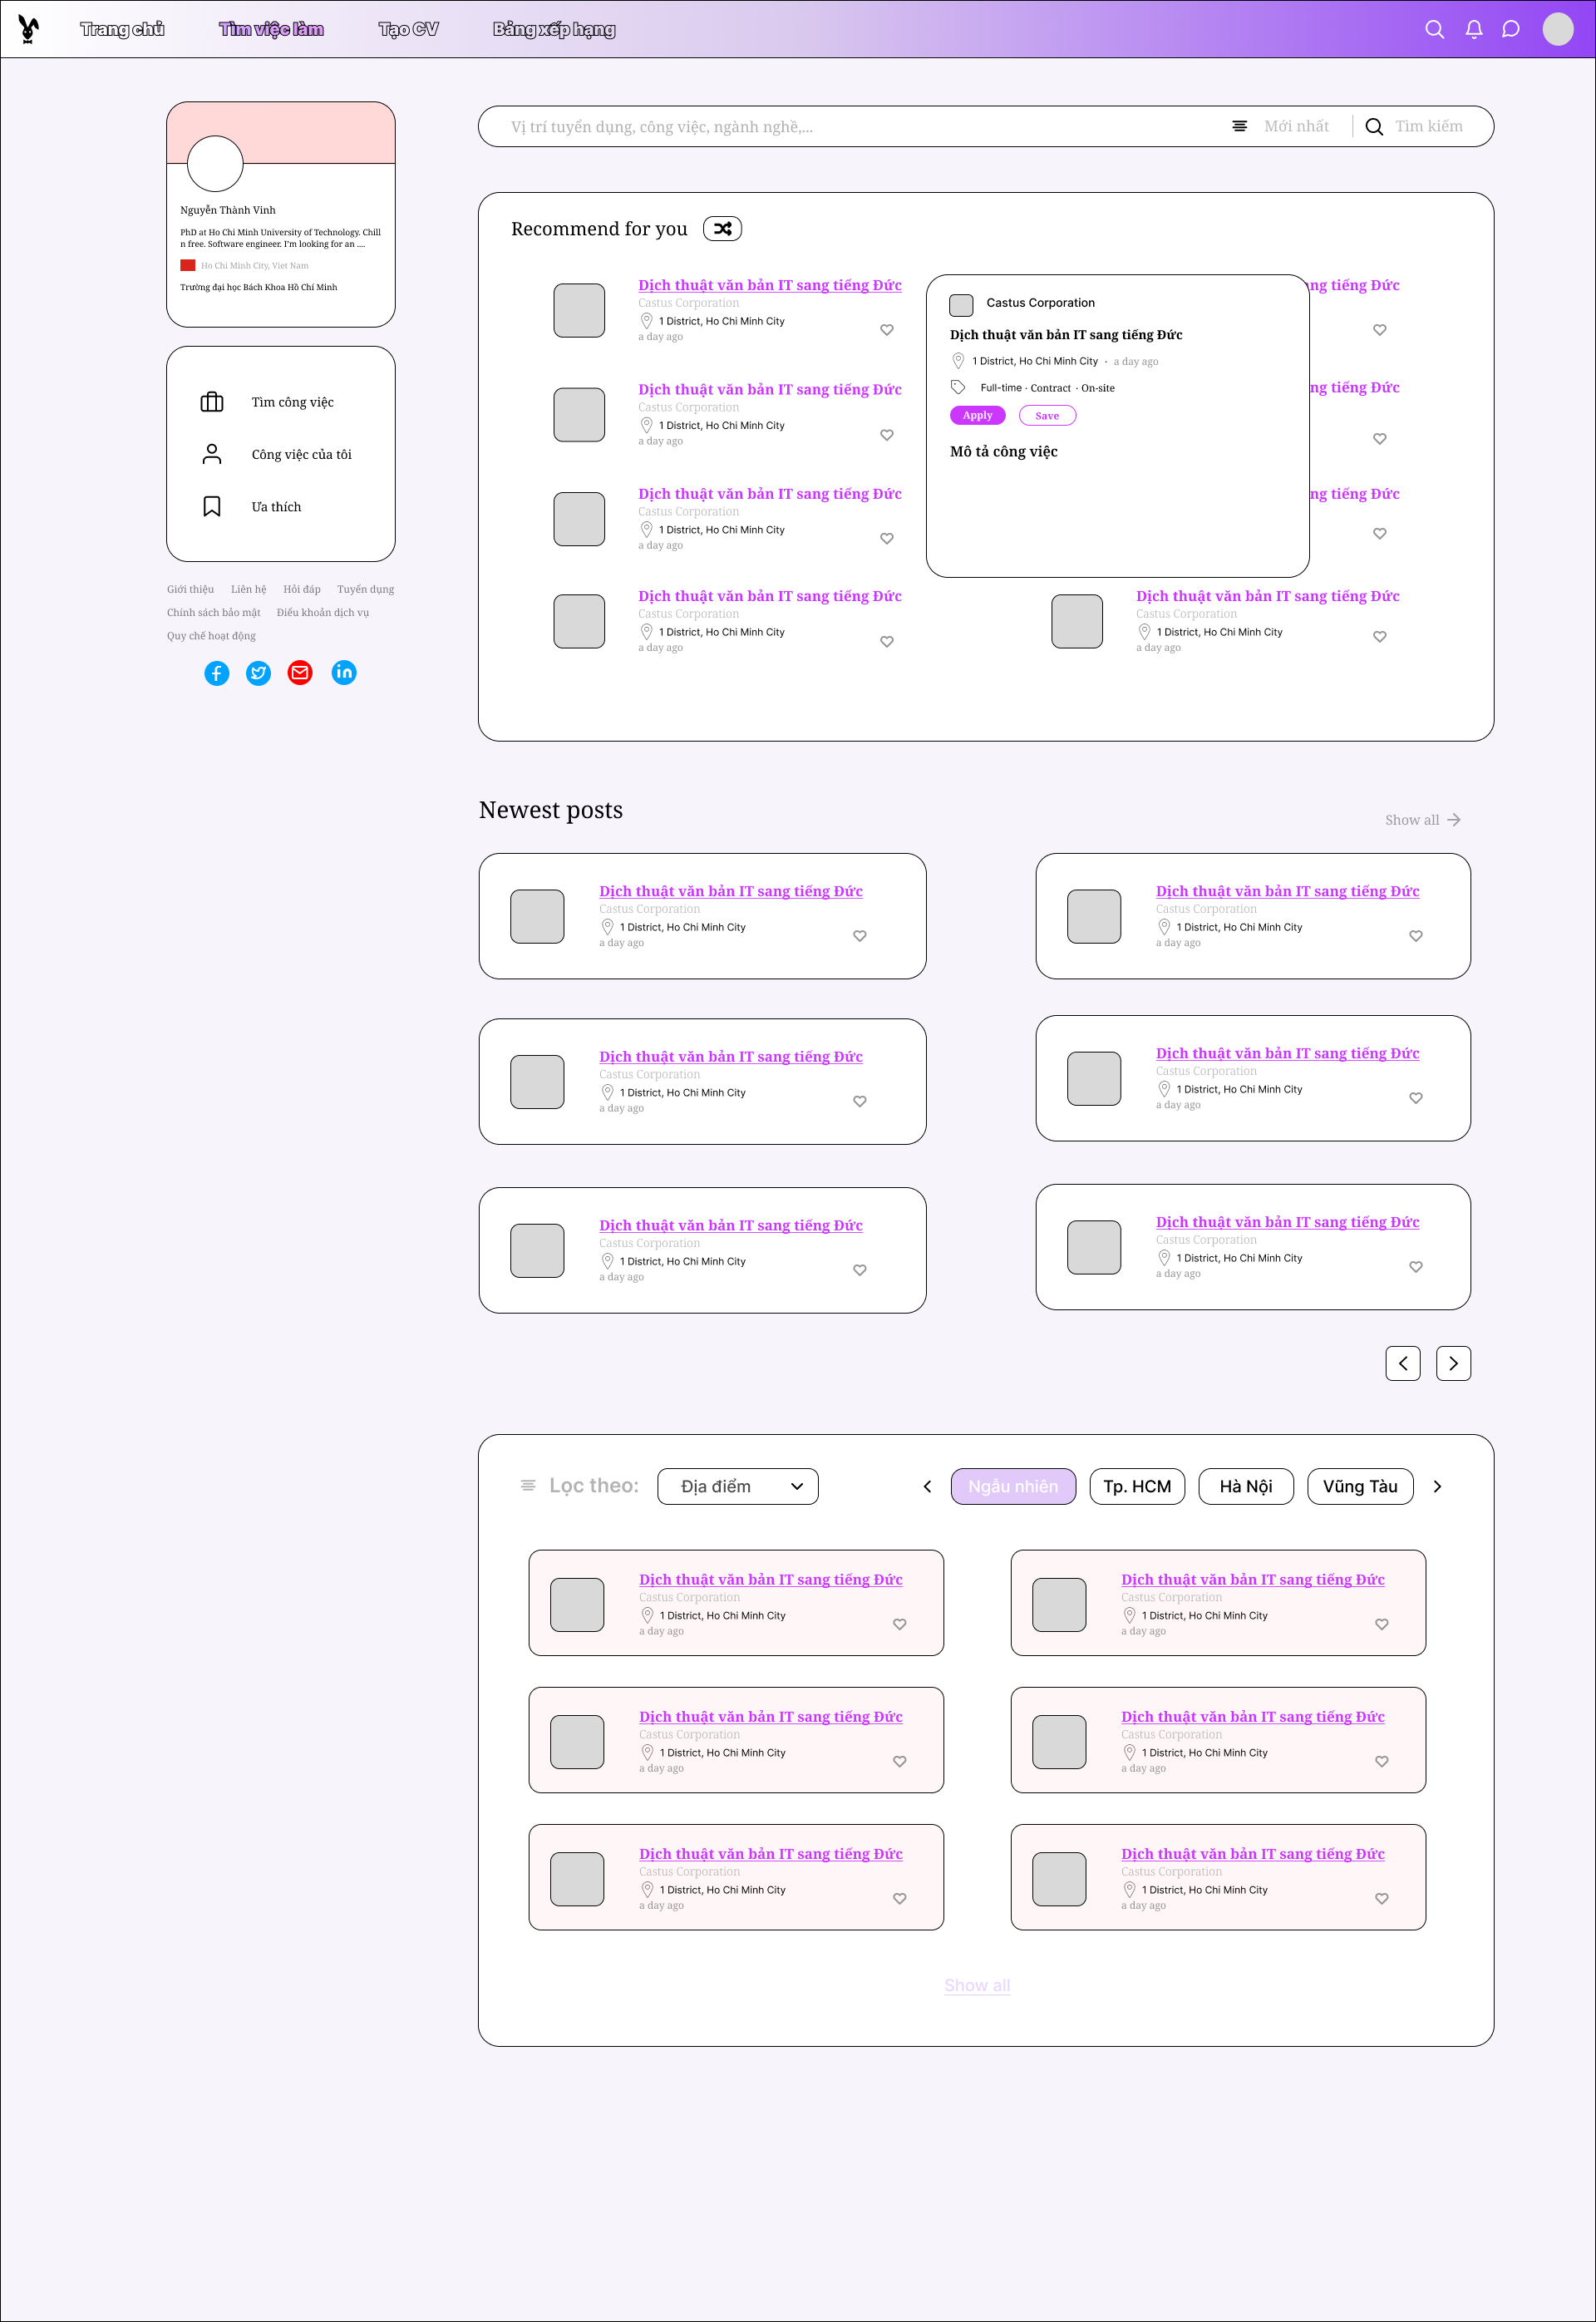
\includegraphics[height=0.58\textheight,trim=0 560 0 0,clip]{img/FindingJob.png}
    \caption{Giao diện tìm kiếm và xem nhanh việc làm}
    \label{fig:finding-job}
\end{figure}

Người dùng đã xác thực có thể nộp Resume đã lưu hoặc tải một PDF mới qua hai endpoint ứng tuyển tương ứng. Trước khi ghi dữ liệu, backend xác nhận tài khoản, quyền sở hữu CV, trạng thái và hạn của Job. Unique index trên cặp \texttt{jobId}--\texttt{candidateId} là lớp bảo vệ cuối cùng chống ứng tuyển trùng, kể cả khi hai request đến gần nhau. API hiện chưa kiểm tra rõ vai trò phải là ứng viên; đây là điểm cần hoàn thiện thay vì chỉ dựa vào điều hướng frontend.

Application lưu \texttt{jobSnapshot} gồm các thông tin cần thiết của tin tại thời điểm nộp. Nhờ đó, lịch sử ứng tuyển vẫn có ngữ cảnh nếu doanh nghiệp xóa Job. Với PDF upload hợp lệ, backend tạo Resume ảo và liên kết với Application; Resume này không xuất hiện trong danh sách CV quản lý thường ngày.

\section{Cổng doanh nghiệp}

Doanh nghiệp dùng chung cơ chế xác thực nhưng có bố cục và route riêng. Các chức năng đã triển khai gồm:

\begin{itemize}
    \item cập nhật hồ sơ công ty;
    \item tạo tin nháp, đăng hoặc chỉnh sửa tin;
    \item bật hoặc tắt nhận hồ sơ và xóa tin;
    \item xem danh sách ứng viên;
    \item cập nhật trạng thái Application.
\end{itemize}

Trạng thái hồ sơ gồm Pending, Reviewing, Interview, Offered, Rejected và Accepted. Form tin tuyển dụng bổ sung kinh nghiệm, học vấn, mô hình làm việc và kiểm tra hạn tối đa hai năm. Tuy nhiên, trạng thái xác minh doanh nghiệp chưa được kiểm tra tại endpoint tạo tin, nên quy trình duyệt chưa phải một cổng cưỡng chế hoàn chỉnh.

Khi doanh nghiệp yêu cầu xem CV, backend không chỉ kiểm tra role company mà còn kiểm tra Job/Application liên quan. Khi trạng thái Application thay đổi, hệ thống tạo Notification cho ứng viên. Cơ chế này liên kết thao tác tuyển dụng với lịch sử và thông báo, thay vì để từng màn hình thay đổi dữ liệu độc lập.

\section{Chat và thông báo}

Chat sử dụng mô hình ``lưu trước, phát sau''. Client gửi nội dung qua REST API; backend lấy danh tính người gửi từ JWT, kiểm tra có văn bản hoặc ảnh, lưu Message rồi phát sự kiện \texttt{newMessage} đến phòng của người nhận bằng Socket.IO. Nếu ghi cơ sở dữ liệu thất bại, server không phát một thông điệp chưa tồn tại. Văn bản được React hiển thị như chuỗi; ảnh được CompressorJS nén ở client trước khi chuyển thành data URL. Backend hiện chưa áp dụng giới hạn loại/dung lượng ảnh và chưa xác minh đầy đủ người gửi thuộc phòng riêng, vì vậy không gọi đây là luồng đã được làm sạch hoàn toàn.

ChatReadState lưu \texttt{lastReadAt} theo người dùng và phòng để chỉ báo chưa đọc tồn tại qua lần tải lại. HiddenChat cho phép một người ẩn cuộc hội thoại khỏi danh sách của mình mà không xóa Message của phía còn lại; tin mới sau mốc ẩn có thể làm phòng xuất hiện lại. Notification là collection riêng, hỗ trợ phân trang, đếm chưa đọc, đánh dấu từng mục hoặc tất cả và xóa. Hook thông báo dùng TanStack Query để cache các trang, cập nhật trạng thái đọc trước trên giao diện và truy vấn số chưa đọc mỗi 30 giây; message dùng kết nối thời gian thực.

\section{Khu vực quản trị}

Backend cung cấp các nhóm chức năng quản trị sau:

\begin{itemize}
    \item thống kê và chẩn đoán health chi tiết;
    \item xem danh sách, ẩn, hiện hoặc xóa Job;
    \item xem danh sách và xác minh doanh nghiệp;
    \item khóa hoặc xóa User.
\end{itemize}

Các endpoint này dùng xác thực và kiểm tra vai trò admin. Frontend hiện chỉ giữ các màn hình có API thật gồm dashboard, người dùng, việc làm và doanh nghiệp; các đường dẫn báo cáo, đánh giá và nhật ký cũ chuyển về trang hợp lệ. Endpoint khóa User hiện chỉ đặt trạng thái khóa, chưa có thao tác mở lại tương ứng cho tài khoản thông thường. Vì vậy báo cáo ghi nhận quản trị ở mức cơ bản, không xem toàn bộ khu vực admin là hoàn tất.

\section{Bảo mật và giới hạn triển khai}

Các lớp bảo vệ chính trong quá trình triển khai gồm:

\begin{itemize}
    \item \textbf{HTTP header:} Helmet thiết lập CSP, chặn nhúng trang và đặt chính sách referrer; cấu hình Vercel bổ sung các header về quyền truy cập thiết bị, kiểu nội dung và tài nguyên chéo nguồn.
    \item \textbf{Nguồn truy cập và tần suất:} CORS chỉ cho các origin được cấu hình; API chung chịu giới hạn 300 yêu cầu trong 15 phút, đăng nhập tối đa 10 lần thất bại trong 15 phút, đăng ký tối đa 10 lần mỗi giờ và AI có giới hạn riêng.
    \item \textbf{Dữ liệu phản hồi:} các danh sách trường \texttt{SELF\_USER\_FIELDS}, \texttt{PUBLIC\_USER\_FIELDS} và \texttt{ADMIN\_USER\_FIELDS} giới hạn dữ liệu tài khoản được trả theo từng ngữ cảnh; mật khẩu và mã PIN không được đưa vào phản hồi.
\end{itemize}

Các biện pháp trên là lớp bảo vệ cơ bản, chưa phải chứng nhận an toàn. Khi thiếu biến môi trường, mã nguồn vẫn có khóa JWT dự phòng; kết nối cơ sở dữ liệu còn tự tạo tài khoản quản trị trình diễn với mật khẩu ngắn. Hai hành vi này thuận tiện cho phát triển nhưng không phù hợp production. Ngoài ra cần hoàn thiện kiểm tra vai trò cho AI/ứng tuyển/lưu việc, xác minh thành viên phòng chat ở mọi thao tác, CSRF, chính sách mật khẩu, giới hạn ảnh, nhật ký kiểm toán và quy trình xoay bí mật.

\section{Cấu hình và khả năng vận hành}

Trong môi trường phát triển, Vite phục vụ frontend và proxy request \texttt{/api} cùng \texttt{/socket.io} đến backend Express. Script \texttt{start:all} điều phối hai tiến trình; Nodemon chỉ theo dõi backend và tệp môi trường để build frontend không gây khởi động lại máy chủ. Backend đọc URI MongoDB, tên cơ sở dữ liệu, JWT secret, nguồn frontend, cấu hình AI và khóa cron từ biến môi trường. Tên biến và quy trình chạy được tổng hợp ở Phụ lục A; báo cáo không ghi giá trị bí mật.

Tệp \texttt{vercel.json} định tuyến API và Socket.IO đến Express, phục vụ ứng dụng một trang, đặt security header và khai báo lịch \texttt{0 0 * * *} cho endpoint hạn tin. Lệnh build Vite tạo được sản phẩm frontend production với các nhóm mã tách riêng. Kết quả này xác nhận mã có thể đóng gói, nhưng không đồng nghĩa hệ thống đã được đánh giá tải, HTTPS, cơ sở dữ liệu production, độ bền Socket.IO serverless hoặc quy trình khôi phục sự cố. Triển khai thực tế cần bí mật mạnh, CORS đúng nguồn, cookie Secure, quan sát log và chiến lược lưu tệp ngoài MongoDB.

\section{Đối chiếu yêu cầu với hiện thực}

\begin{table}[H]
    \centering
    \small
    \begin{tabularx}{\textwidth}{|p{0.20\textwidth}|p{0.29\textwidth}|Y|} \hline
        \textbf{Nhóm yêu cầu} & \textbf{Bằng chứng triển khai} & \textbf{Điểm cần xác minh ở Chương 7} \\ \hline
        FR-CV, FR-AI & Resume, A4/PDF, năm route AI, AiUsage & Layout A4, PDF validation, sanitizer và hợp đồng AI. \\ \hline
        FR-JOB, FR-APP & Job, Application, saved jobs, unique index, snapshot & Hạn tin, trùng hồ sơ, lịch sử và dữ liệu PDF. \\ \hline
        FR-COM & Route Job/Application và layout doanh nghiệp & Trạng thái hồ sơ, quyền xem CV và notification. \\ \hline
        FR-MSG & Message, Socket.IO, ChatReadState, HiddenChat & Rich text, badge chưa đọc và trạng thái theo user. \\ \hline
        FR-ADM & Admin routes và dashboard & Ma trận quyền cùng sự tương ứng frontend--backend. \\ \hline
    \end{tabularx}
    \caption{Truy vết từ yêu cầu sang thành phần triển khai}
    \label{tab:implementation-traceability}
\end{table}
